\begin{figure}[!h]
  %\centering
  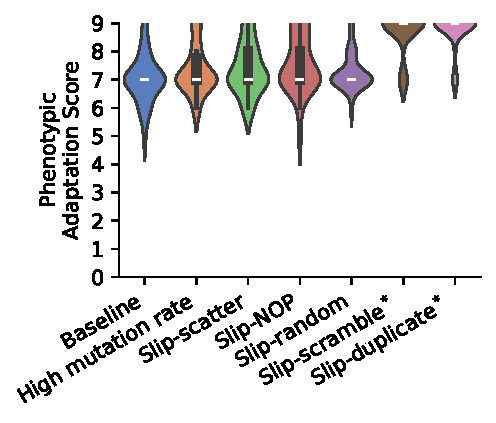
\includegraphics[height=2in,trim={0.2cm 0 0.2cm 0},clip]{binder/binder/teeplots/env=static+hue=treatment+inner=box+kind=violin+palette=muted+viz=catplot+x=treatment+y=tasks-present+ext=.pdf}%
   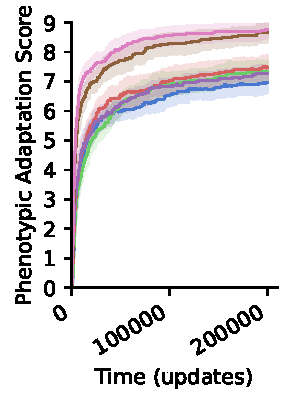
\includegraphics[height=2in,trim={0.94cm -0.64cm 0 0},clip]{binder/binder/teeplots/env=static+errorbar=ci+hue=treatment+kind=line+palette=muted+viz=relplot+x=time+y=tasks-present+ext=.pdf}

   \vspace{-2ex}

  \caption{\textbf{Slip-scramble and slip-duplicate treatments facilitate adaptive evolution.}
  \small Violin plots indicate the phenotypic match scores for final dominants.
  Each time series shows the phenotypic match scores for the lineages of final dominant organisms over time. The colors in each time series correspond to the colors in the violin plots.
  Treatments that have significantly higher phenotypic match scores than the baseline treatment are marked with *.
  Data shown from second-phase experiments.
}
  \label{fig:results_panels}
\end{figure}
